\chapter{Реализация и использование}\label{implementation}
\section{Реализованные методы анализа экспрессии}
\subsection{Метод главных компонент и визуализация его результата}
Данный инструмент предназначен для построения графиков в соответствие с методом главных компонент.
В качестве аргументов на вход к инструменту подается:
\begin{itemize}
\item номера образцов для сравнения;
\item категориальная аннотация для различения точек по цвету (если не указана, то стандартный цвет);
\item числовая аннотация для различения точек по размеру (если не указана, то стандартный размер);
\item аннотация для подписей к точкам (если не указана, то без подписи);
\item функция замены \texttt{NA} в данных при вычислении матрицы \emph{PCA} (\texttt{mean} или \texttt{median}).
\end{itemize}

\begin{figure}[h]
  \caption{Инструмент \texttt{PcaPlotTool} и отрисованный график по данным GSE14308}
  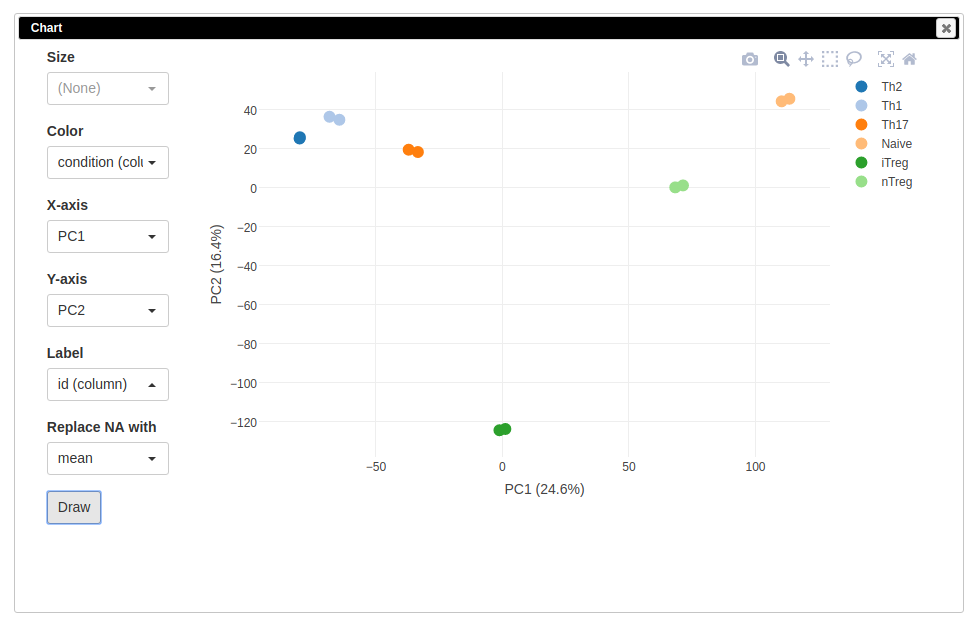
\includegraphics[scale=0.4]{plotexample.png}
  \label{plotexample}
\end{figure}

Далее по алгоритму, описанному в разделе~\ref{functioncallalgo}, на \emph{OpenCPU}-сервер отправляется \emph{RPC}-вызов с аргументами: ключ сессии, содержащий актуальный \texttt{ExpressionSet}, и функция замены \texttt{NA}. На клиент в \emph{JSON}-формате приходит вычисленная матрица \emph{PCA}.

После, по дополнительным аргументам и вычисленной матрице, строится интерактивный график с помощью \emph{plotly.js}, пример которого можно увидеть на рисунке~\ref{plotexample}.

\subsection{Кластеризация методом kmeans}
Этот инструмент осуществляет разбиение генов на указанное пользователем число кластеров по алгоритму \emph{kmeans}.

\begin{figure}[h]
  \caption{Графический интерфейс инструмента \texttt{KmeansTool}}
  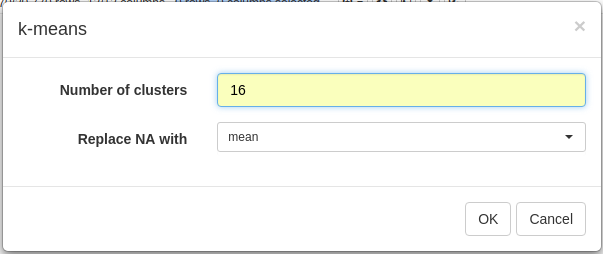
\includegraphics[scale=0.4]{kmeanstool.png}
   \label{kmeanstool}
\end{figure}

На клиенте в инструменте \texttt{KmeansTool}, который показан на рисунке~\ref{kmeanstool}, считываются следующие аргументы:
\begin{itemize}
\item количество кластеров, на которые нужно разбить данные;
\item функция замены \emph{NA} в данных.
\end{itemize}

Данные аргументы и ключ сессии актуального \texttt{ExpressionSet} отправляются на сервер. На сервер возвращается список соответствия каждого гена определенному кластеру, который отрисовывается как новая цветовая аннотация к строкам, пример такой аннотации можно увидеть на рисунке~\ref{kmeansexample}.
\begin{figure}[h]
  \caption{Результат работы инструмена \texttt{KmeansTool} на данных GSE14308}
  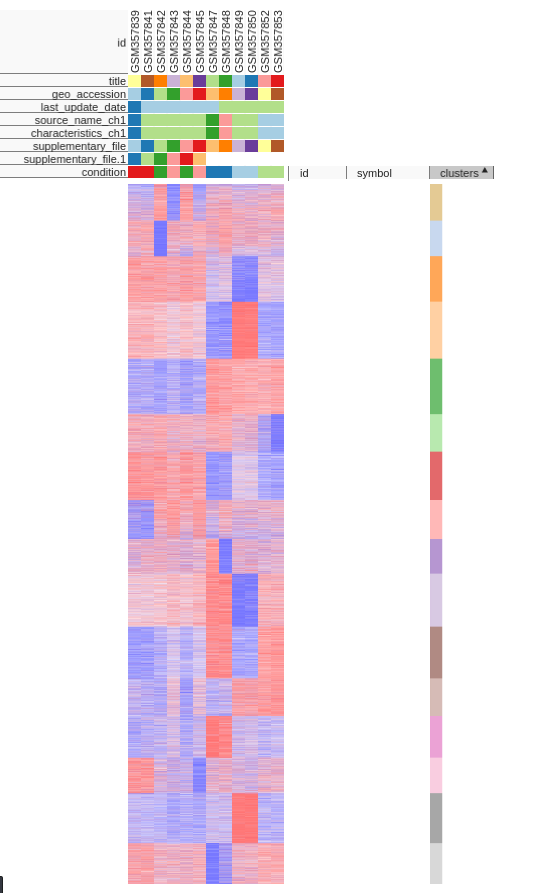
\includegraphics[scale=0.4]{kmeansexample.png}
  \label{kmeansexample}
\end{figure}

\subsection{Анализ дифференциальной экспрессии}
Инструмент предназначен для анализа дифференциальной экспрессии: экспрессия генов сравнивается в двух группах образцов, и вычисляются несколько статистических характеристик, показывающих, насколько случайны различия этих групп.

\begin{figure}[h]
  \caption{Графический интерфейс инструмента \texttt{LimmaTool}}
  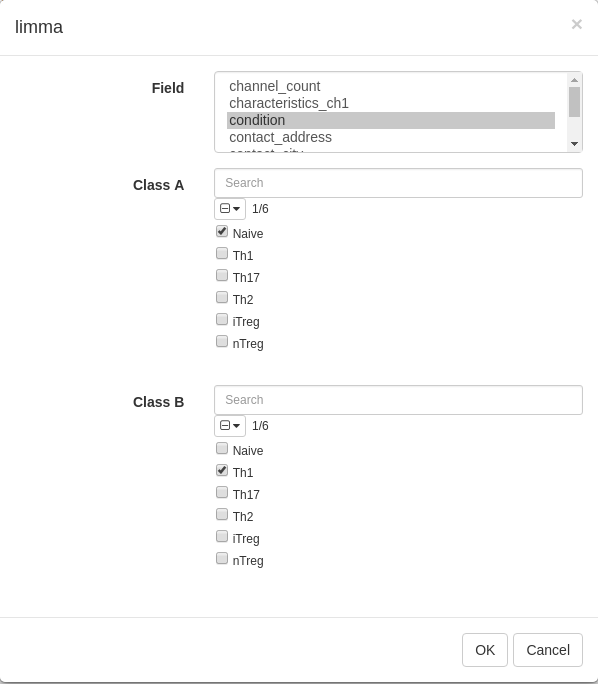
\includegraphics[scale=0.4]{limmatool.png}
  \label{limmatool}
\end{figure}

На клиенте, в инструменте, показанном на рисунке~\ref{limmatool}, осуществляется получение следующих аргументов:
\begin{itemize}
\item какие аннотации образцов участвуют в сравнении;
\item какая комбинация значений указанных выше аннотаций обозначает класс A;
\item аналогично для класса B.
\end{itemize}

Далее происходит подготовка аргументов к отправке на сервер: образцы разбиваются по выбранным аннотациям на три группы: A, B и не участвующие в сравнении.
Список соответствия образцов классам и ключ сессии, содержащей актуальный \texttt{ExpressionSet}, отправляются на сервер.

\begin{figure}[h]
  \caption{Результат работы инструмента \texttt{LimmaTool} на данных GSE14308}
  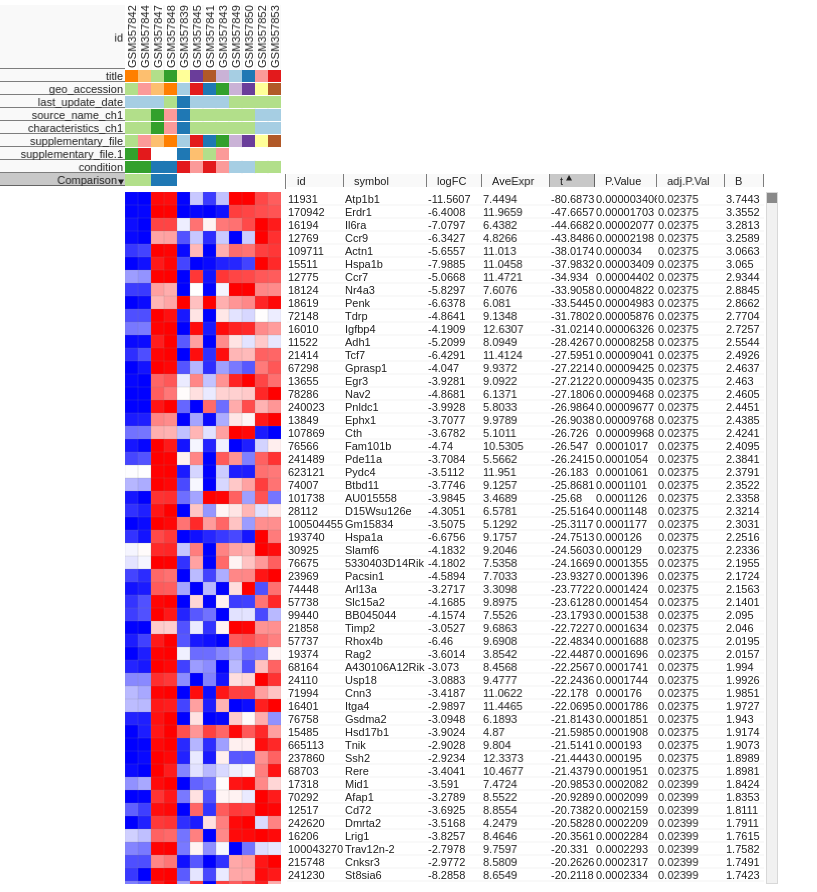
\includegraphics[scale=0.4]{limmaexample.png}
  \label{limmaexample}
\end{figure}

От сервера приходит файл с сериализованной в \emph{ProtoBuf} матрицей результатов, которые с помощью \emph{protobuf.js} разбираются и отрисовываются в виде аннотации к строкам. Результат работы можно увидеть на рисунке~\ref{limmaexample}.
\subsection{Дифференциальная экспрессия --- limmaAnalysis}
\emph{R}-пакет \emph{limma}~\cite{limma} предоставляет методы для вычисления дифференциальной экспрессии. Данная функция помогает увидеть, насколько случайны или нет различия между образцами в генах в разных условиях.

Соответственно, так как данный метод анализа часто применяется в задаче анализа экспрессии генов, было решено включить в \emph{phantasus} поддержку этой функции.

Реализация функции \texttt{limmaAnalysis} в \emph{R}-пакете \emph{phantasus} принимает в себя \texttt{ExpressionSet} и вектор соответствия образцов классам. Класс в этом векторе может быть A, B или пустым (в данном классе находятся образцы, не участвующие в сравнении). Необходимо сравнить классы A и B, а для этого нужно дополнить фенотипические данные \texttt{ExpressionSet} полученным вектором.
После дизайн сравнения передается в функцию, которая возвращает матрицу статистических характеристик к каждому гену.
Эта матрица далее сериализуется в \emph{ProtoBuf}, записывается в файл, который будет в дальнейшем разобран на клиенте.

Код функции \texttt{limmaAnalysis} представлен на листинге~\ref{limmaAnalysis}.

\begin{lstlisting}[float=!h,caption={Реализация дифференциальной экспрессии в R-пакете phantasus},label={limmaAnalysis},language=R]
limmaAnalysis <- function(es, rows = c(), columns = c(), fieldValues) {
  assertthat::assert_that(length(columns) == length(fieldValues) || length(columns) == 0)
  rows <- getIndicesVector(rows, nrow(exprs(es)))
  columns <- getIndicesVector(columns, ncol(exprs(es)))
  fieldName <- "Comparison"
  fieldValues <- replace(fieldValues, fieldValues == '', NA)
  new.pdata <- pData(es)[columns,]
  new.pdata[[fieldName]] <- as.factor(fieldValues)
  new.pdata <- new.pdata[!is.na(new.pdata[[fieldName]]),]
  new.sampleNames <- row.names(new.pdata)
  es.copy <- es[rows, new.sampleNames]
  pData(es.copy) <- new.pdata
  fData(es.copy) <- data.frame(row.names=rownames(es.copy))
  es.design <- model.matrix(~0 + Comparison, data = pData(es.copy))
  colnames(es.design) <- gsub(pattern = fieldName,
                              replacement = '',
                              x = make.names(colnames(es.design)))
  fit <- lmFit(es.copy, es.design)
  fit2 <- contrasts.fit(fit, makeContrasts(B - A,
                                           levels=es.design))
  fit2 <- eBayes(fit2)
  de <- topTable(fit2, adjust.method="BH", number=Inf)
  de <- de[row.names(fData(es.copy)),]
  f <- tempfile(pattern = "de", tmpdir = getwd(), fileext = ".bin")
  writeBin(protolite::serialize_pb(as.list(de)), f)
  f
}
\end{lstlisting}

\subsection{Загрузка данных из GEO --- loadGEO}
В обзоре были описаны форматы данных в репозитории \emph{Gene Expression Omnibus}.
В \emph{phantasus} загрузка данных из \emph{GEO} осуществляется следующим образом:
\begin{enumerate}
\item функция \texttt{loadGEO} принимает на вход идентификатор \texttt{GEO};
\item в зависимости от его вида (\emph{GSE} или \emph{GDS}) запускаются дополнительные функции (\texttt{getGSE} на листинге~\ref{getGSE} и \texttt{getGDS} на листинге~\ref{getGDS});
\item в каждой из двух функций с помощью \texttt{GEOquery::getGEO} загружаются данные с аннотацией (или подгружаются из кэша, если он указан или если их уже загружали);
\item результат обрабатывается, создается \texttt{ExpressionSet} и отправляется в глобальные переменные;
\item в файл записываются сериализованные в \emph{ProtoBuf} данные, в том же формате, что и при создании \texttt{ExpressionSet} из внешних данных (смотри раздел~\ref{createESsection}), которые после считает и обработает клиент.
\end{enumerate}
\begin{lstlisting}[float=!h,caption={Загрузка данных типа GSE из Gene Expression Omnibus},label={getGSE},language=R]
getGSE <- function(name, destdir = tempdir()) {
  es <- getGEO(name, AnnotGPL = T, destdir = destdir)[[1]]
  featureData(es) <- featureData(es)[,grepl("symbol", fvarLabels(es), ignore.case = T)]
  phenoData(es) <- phenoData(es)[,grepl("characteristics", varLabels(es), ignore.case = T)
                                  | (varLabels(es) %in% c("title", "id", "geo_accession"))]
  chr <- varLabels(es)[grepl("characteristics", varLabels(es), ignore.case = T)]
  take <- function(x, n) {
    sapply(x, function(x) { x[[n]] })
  }
  rename <- function(prevName, x) {
    splitted <- strsplit(x, ": ")
    sumlength <- sum(sapply(as.vector(splitted), length))
    if (sumlength != 2 * length(x)) {
       return(list(name = prevName, x = x))
    }
    splittedFirst <- unique(take(splitted, 1))
    if (length(splittedFirst) == 1) {
       res = list(name = splittedFirst[1], x = take(splitted, 2))
    }
    else {
       res = list(name = prevName, x = x)
    }
    res
  }
  renamed <- lapply(chr, function(x) { rename(x, as.vector(pData(es)[,x])) })
  phenoData(es) <- phenoData(es)[, !(varLabels(es) %in% chr)]
  pData(es)[,take(renamed,1)] <- take(renamed,2)
  es
}
\end{lstlisting}

\begin{lstlisting}[float=!h,caption={Загрузка данных типа GDS из Gene Expression Omnibus},label={getGDS},language=R]
 getGDS <- function(name, destdir = tempdir()) {
  l <- getGEO(name, destdir = destdir)
  table <- slot(l, 'dataTable') # extracting all useful information on dataset
  data <- Table(table)  # extracting table ID_REF | IDENTIFIER/SAMPLE | SAMPLE1 | ...
  columnsMeta <- Columns(table) # phenoData
  sampleNames <- as.vector(columnsMeta[["sample"]])
  rownames <- as.vector(data[["ID_REF"]])
  symbol <- as.vector(data[["IDENTIFIER"]])
  data <- data[,sampleNames] # expression data
  exprs <- as.matrix(data)
  row.names(exprs) <- rownames
  row.names(columnsMeta) <- sampleNames
  # columnsMeta <- columnsMeta[,!(colnames(columnsMeta) %in% c('sample'))] 
  pData <- AnnotatedDataFrame(data.frame(columnsMeta, check.names = F))
  fData <- data.frame(matrix(symbol, nrow(exprs), 1));
  colnames(fData) <- "symbol"
  fData <- AnnotatedDataFrame(fData)
  featureNames(fData) <- rownames
  ExpressionSet(assayData = exprs, phenoData = pData, featureData = fData)
}
\end{lstlisting}

Основной код загрузки и дополнительные утилиты к нему можно увидеть на листинге~\ref{loadGEO}.

\begin{lstlisting}[float=!h,caption={Загрузка данных из Gene Expression Omnibus},label={loadGEO},language=R]
loadGEO <- function(name, type = NA) {
  es <- getES(name, type, destdir = "/var/phantasus/cache")
  assign("es", es, envir = parent.frame())
  data <- as.matrix(exprs(es)); colnames(data) <- NULL; row.names(data) <- NULL

  pdata <- as.matrix(pData(es)); colnames(pdata) <- NULL; row.names(pdata) <- NULL

  participants <- colnames(es)
  rownames <- rownames(es)

  fdata <- as.matrix(fData(es))
  colnames(fdata) <- NULL
  row.names(fdata) <- NULL

  res <- list(data = data, pdata = pdata,
              fdata = fdata, rownames = rownames,
              colMetaNames = varLabels(phenoData(es)),
              rowMetaNames = varLabels(featureData(es)))

  f <- tempfile(pattern = "gse", tmpdir = getwd(), fileext = ".bin")
  writeBin(protolite::serialize_pb(res), f)
  f
}
getES <- function(name, type = NA, destdir = tempdir()) {
  if (is.na(type)) {
     type = substr(name, 1, 3)
  }
  if (type == 'GSE') {
    es <- getGSE(name, destdir)
  }
  else if (type == 'GDS') {
    es <- getGDS(name, destdir)
  }
  else {
    stop("Incorrect name or type of the dataset")
  } 
  es
}
\end{lstlisting}


\section{Структура git-репозитория}
Как следует из главы об архитектуре проекта, проект состоит из двух составляющих:
\begin{itemize}
\item phantasus.js --- fork репозитория morpheus.js \cite{morpheus};
\item phantasus --- репозиторий для R-пакета.
\end{itemize}
Внутри репозитория phantasus находится подмодуль для репозитория phantasus.js.
Соответственно, чтобы загрузить целиком весь проект достаточно вызвать команду из листинга~\ref{clonerepo}.
\begin{lstlisting}[float=!h,language=bash,label={clonerepo},caption={Клонирование репозитория проекта phantasus}]
  git clone --recursive https://github.com/ctlab/phantasus.git
\end{lstlisting}

\section{Кэш для данных из GEO}
Независимо от способа запуска, данные, загруженные из GEO, кэшируются в определенной папке, чтобы не было необходимости перескачивать их заново.

\section{Единый R-пакет phantasus}
Так как проект теперь существует в виде почти единого git-репозитория, его легко можно использовать как полноценный R-пакет, содержащий в себе в том числе и файлы для веб-приложения.
С помощью функции, представленной на листинге~\ref{serve.R}, можно запускать веб-приложение phantasus непосредственно из R.
\lstinputlisting[float=!h,language=R,label={serve.R},caption={Функция для запуска приложения из R}]{listings/serve.R}

\section{Docker-образ phantasus}
На hub.docker.com существует автоматический репозиторий, привязанный к git-репозиторию phantasus. Для каждой перекомпиляции он использует Dockerfile с листинга~\ref{dockerfile}, расположенный в репозитории.

На данный момент существуют две ветки Docker-образа:
\begin{itemize}
\item master --- компиляция происходит из master-веток составляющих проекта, чаще всего эти скомпилированные образы стабильны и отправляются в открытый доступ для использования;
\item develop --- компиляция происходит из develop-веток составляющих проекта, эти образы используются для тестирования всего приложения в целом, тестирования нового функционала и не предназначены для использования на серверах.
\end{itemize}

Чтобы загрузить Docker-образ, нужно воспользоваться командой с листинга~\ref{dockerpull}
\begin{lstlisting}[float=!h,language=bash,label={dockerpull},caption={Загрузка Docker-образа phantasus}]
  docker pull dzenkova/phantasus
\end{lstlisting}

\subsection{Запуск Docker-контейнера}

\section{Настройка с помощью Apache}
\subsection{Переадресация OpenCPU-сервера}
После того, как сравнили скорость работы с использованием single-user OpenCPU-сервера и multi-user, пришли к выводу, что скорость доступа к первому выше из-за того, что RApache работает достаточно медленно.

Соответственно, происходит переадресация запросов с /ocpu на //localhost:8001/ocpu.
\subsection{Балансировщик для multi-user соединения}
Из-за того, что используется single-user OpenCPU-сервер, несколько людей, использующих веб-приложение phantasus одновременно, вынуждены ждать, пока закончится запрос для одного.

Чтобы такого не происходило, запускается четыре экземпляра OpenCPU-сервера и с помощью Apache-балансировщика можно получать доступ к R-серверу параллельно.

\section{Статистика использования}

\chapterconclusion
В данной главе были рассмотрены технические подробности реализации веб-приложения: инструкции для запуска, варианты использования и подробности настройки веб-приложения на сервере.
